\section{Path Co-Width: An Alternative Definition via a Grammar}\label{appendix: grammar}
In what follows, we reformulate the definition of path co-width for \textit{symmetric graphs} so that it is easier to analyse inductively.
For $k\in\mathbb{N}$, a \define{$(\le k)$-coloured graph} is a graph $G$ along with an assignment $\lambda \colon V(G) \to \{1, \dots, k\}$ of colours to the vertices (these are not proper colourings). We define the following two operations on $(\le k)$-coloured graphs -- the ideas are simple, but aiming for maximum clarity, slightly verbose, bare with us: 
\begin{enumerate}
    \item \define{Colour merging.} Picking colors $i$ and $j$, define the $(\le k)$-coloured graph $(i \to j)(G, \lambda) := (G, \lambda')$ where $\lambda'$ recolors colour class $i$ to colour class $j$; formally we have
    \[\lambda' \colon x \mapsto \begin{cases} j &\text{if } \lambda(x) = i \\ 
    \lambda(x) &\text{otherwise}.\end{cases}\]
    \item \define{Class splitting.} This operation can only be performed when $G$ is colored with exactly $k'$ colors where $k' < k$. The rough idea is that, picking a color $i$, we will duplicate this color class and then join edges between these copies to the other color classes according to some simple rules (see Figure~\ref{fig:grammar} to get a feeling). Since this involves keeping track of various adjacencies, we will end up storing this data as a matrix. We need some notation. Denote the induced subgraph on $\lambda(i)^{-1}$ as $C_i$. Given a choice of a color $i$, a \define{class-$i$ splitting matrix} $A(i)$ is a binary matrix whose rows and columns are indexed as 
    \[
        \begin{array}{c|cccc|cc|c}
            & C_1 & C_2 & \cdots & C_{i-1} & C_i^1 & C_i^2 & C_{i+1} \; \cdots \; C_{k'} \\
            \hline
            C_i^1   &  &  &  &  & E_{i}^{11} & E_i^{12} &  \\
            C_i^2  &  &  &  &  & E_i^{21} & E_i^{22} &  
        \end{array}
    \]
    and satisfying the following conditions: 
    \begin{enumerate}
        \item every row indexed by some $j \neq i$ is a non-zero vector and 
        \item the block matrix  
            \(
                \begin{pmatrix}
                    \cdots & \big| & E_{i}^{11} & E_i^{12} & \big| & \cdots \\
                    \cdots & \big| & E_i^{21} & E_i^{22} & \big| & \cdots
                \end{pmatrix}
            \) is non-zero and $E_i^{21} = E_i^{12}$. 
    \end{enumerate}
    Given this matrix, we can finally define the class splitting operation, which we denote $A(i)(G, \lambda)$. This is the graph obtained as follows (see Figure~\ref{fig:grammar}):
    \begin{itemize}
        \item let $G'$ be the graph obtained by replacing $C_i$ with two copies $C_i^1$ and $C_i^2$ having the same adjacencies both within and outwith their color class  
        \item for each $h \in \{1, 2\}$, delete all edges between $C_i^h$ and $C_j$ if the         \item for each $h \in \{1, 2\}$, delete all edges between $C_i^h$ and $C_j$ if the $(C_i^h, C_j)$-th entry of $A(i)$ is zero; similarly delete all edges between $C_i^h$ and $C_i^g$ -- where $g \in \{1, 2\}$ -- if the $(C_i^h, C_i^g)$-th entry of $A(i)$ is zero (if $g = h$, then this amounts to removing all edges within the induced subgraph $C_i^h$).
        \item we obtain a $k' + 1$ coloring by adding a new color class for $C_{i}^2$ and leaving all other color classes the same (in particular $C_{i}^1$ retains color $i$).
    \end{itemize}
    \end{enumerate}
Define the \define{class of $(\le k)$-coloured graphs $\mathbb{C}_k$} recursively as follows:
\begin{enumerate}
    \item every $(\le k)$-coloured graph on $\le k$ vertices is in $\mathbb{C}_k$; and
    \item if $(G,\lambda)\in\mathbb{C}_k$, then the graph obtained from $(G,\lambda)$ by merging colour classes is in $\mathbb{C}_k$; and
    \item if $(G,\lambda)\in\mathbb{C}_k$ and $(G,\lambda)$ uses strictly less than $k$ colours, then the graph obtained from $(G,\lambda)$ by class splitting is in $\mathbb{C}_k$.
\end{enumerate}

\begin{figure}
    \centering
    \tikzfig{grammar}
    \caption{On the left we have a colored graph $(G, \lambda)$ with two color classes $i$ and $j$. We will apply the color splitting operation at $i$ with matrix 
    \(
    A(i) = \bigl(\begin{smallmatrix}
    1 & 1 & 1 \\
    0 & 1 & 0
    \end{smallmatrix}\bigr)
    \)
    where rows are indexed by $C_i^1$ and $C_i^2$ and columns are indexed by $C_j$, $C_i^1$ and $C_i^2$. We obtain a graph -- the one on the far right -- in two steps: (1) first we duplicate the color class $i$ and copying all edges and (2) we then delete edges between color classes whenever the matrix $A(i)$ has a zero entry.}
    \label{fig:grammar}
\end{figure}

We will prove that the class $\mathbb{C}_k$ defined by the grammar above captures precisely the graphs of path co-width at most $k$. To do this, we will first need the notion of \textit{gradual} tree co-decompositions which are roughly tree co-decompositions in which each cospan is making only small changes. 

\begin{definition}\label{def: gradual tree co-decomp}
    We say that a tree co-decomposition $\Ta = (T,\{G_a\},\{g_t^e\})$ of a graph $G$ is \define{gradual} if for every cospan $G_i \xrightarrow{g_i^e} G_e \xleftarrow{g_j^e} G_j$ we have that: (1) the difference in the number of vertices of $G_i$ and $G_j$ is at most one and (2) at least one of $g_i^e$ and $g_j^e$ is an identity.
\end{definition}

\begin{lemma}\label{lemm:helper}
    Let $k\in \mathbb{N}$ and $\Ta=(T,\{G_a\},\{g_t^e\})$ be a tree co-decomposition with limit~$G$,  width~$k$ and $n$ bags. Then there exists a gradual tree co-decomposition~$\Ta'$ such that: (1) it has $G$ as its limit (2) it has width at most $k$ and (3) it has at most $2kn$ bags. 
\end{lemma}
\begin{proof}
    Let $G_i\xrightarrow{g_i^e}G_e\xleftarrow{g_j^e} G_j$ be one of the cospans in $\Pa$. Suppose that $G_i$ has at least two vertices more than $G_e$. We observe that we can replace the cospan by the double cospan
    \[
        G_i\xrightarrow{{g_i^e}'} G_i'\xleftarrow{\cat{id}} {G_i}'\xrightarrow{{g_i^e}''}G_e\xleftarrow{g_j^e}G_j
    \]
    where ${g_i^e}'$ performs the identification of a single pair of vertices and ${g_i^e}''$ is such that $g_i^e={g_i^e}''\circ {g_i^e}'$. This new path co-decomposition retains the limit $G$, since pullbacks along identities are identities and thus the original path co-decomposition can be recovered as a partial evaluation at the cospan $G_i\xrightarrow{{g_i^e}'} G_i'\xleftarrow{\cat{id}} G_i'$. Since, by this reasoning, we need to replace each cospan with at most $2k$ cospans, the bound on the number of bags follows.
\end{proof}

We will now show that the graphs obtained our grammar are equivalent to graphs given by gradual path co-decompositions. 

\begin{lemma}
    For $k\in\mathbb{N}$, the class of graphs of path co-width $k$ is the class of underlying (i.e. uncolored) graphs of the graphs in $\mathbb{C}_k$.
\end{lemma}
\begin{proof}
    Let $\Pa=(P,\{G_a\},\{g_t^e\})$ be a path co-decomposition of width $k$. By Lemma~\ref{lemm:helper}, we may assume that $\Pa$ is gradual. Label the vertices of $P$ by $1,\ldots,n$ in the path order. Let $G[i]$ be the limit of the restriction of $\Pa$ to the first $i$ bags and \[g[i] \colon G[i] \twoheadrightarrow G_{i,i+1}\] be the epimorphism produced by the partial evaluation process -- in the diagram below, this is the composite of the $g_i$ (blue) and $g_i^{i+1}$ (orange) arrows below. 
   \begin{center}
\begin{adjustbox}{width=\textwidth}
\begin{tikzcd}[sep=small]
    &&&&& {G[i+1]} &&&&&& \\
    &&& {G[i]} \\
    \\
    {G_1} && {G_2} & \dots & {G_{i-1}} && {G_i} && {G_{i+1}} & \dots & \dots & {G_n} \\
    & {G_{1,2}} && \dots && {G_{i-1, i}} && {G_{i, i+1}} && {G_{i+1, i+2}} & \dots
    \arrow[from=1-6, to=2-4]
    \arrow["{g_{i+1}}", color={rgb,255:red,0;green,153;blue,64}, from=1-6, to=4-9]
    \arrow[color={rgb,255:red,92;green,92;blue,214}, two heads, from=2-4, to=4-1]
    \arrow[color={rgb,255:red,92;green,92;blue,214}, two heads, from=2-4, to=4-3]
    \arrow[color={rgb,255:red,92;green,92;blue,214}, two heads, from=2-4, to=4-5]
    \arrow["{g_i}", color={rgb,255:red,92;green,92;blue,214}, two heads, from=2-4, to=4-7]
    \arrow[two heads, from=4-1, to=5-2]
    \arrow[two heads, from=4-3, to=5-2]
    \arrow[two heads, from=4-3, to=5-4]
    \arrow[two heads, from=4-5, to=5-4]
    \arrow[two heads, from=4-5, to=5-6]
    \arrow[two heads, from=4-7, to=5-6]
    \arrow["{g_i^{i,i+1}}", color={rgb,255:red,214;green,153;blue,92}, two heads, from=4-7, to=5-8]
    \arrow[two heads, from=4-9, to=5-8]
    \arrow["{g_i^{i+1, i+2}}", color={rgb,255:red,120;green,48;blue,192}, from=4-9, to=5-10]
    \arrow[from=4-12, to=5-11]
\end{tikzcd}
\end{adjustbox}
\end{center}
    Let $\Pa[i]=(P,\{G[i],G_{i+1},G_{i+2},\ldots,G_n\},\{g[i]\}\cup\{g_t^e\})$ be the partial evaluation of $\Pa$ obtained by contracting the first $i-1$ edges in the auxiliary path $P$. 
    
    %By associating each of the vertices of $G_{i,i+1}$ (the adhesion between $G_i$ and $G_{i+1}$) 
    For each $i\in [n-1]$, let $(G[i],g[i])$ be the $(\le k)$-coloured graph obtained from $G[i]$ by colouring each vertex by its image under $g[i]$. Let $g[n]$ simply be the projection of $G[n]=G$ into $G_n$ (as if there is an additional adhesion map $g_{n}^{n,n+1}=\cat{id}_{G_n}$). We will prove by induction on $i\in[n]$ that $(G[i],g[i])$ is in the class $\mathbb{C}_k$.

    For the base case, we observe that $G[1]=G_1$ which has at most $k$ vertices. Hence the $(\le k)$-coloured graph $(G[1],g[1])$ is in $\mathbb{C}_k$ by definition. Now assume that $(G[i],g[i])\in \mathbb{C}_k$ for some $i\in[n]$.

    Suppose first that the adhesion $G_{i,i+1}$ and the bag $G_{i+1}$ are the same size, and hence are isomorphic. Then $G[i+1]=G[i]$ and $(G[i+1],g[i+1])$ is the $(\le k)$-coloured graph obtained from $(G[i],g[i])$ by colour merging according the the composite $g_{i+1}^{i+1,i+2}\circ g[i]$.
    
    Now suppose that $G_{i+1}$ has one more vertex than $G_i$. For the vertices of $G_{i+1}$, we write $v_1,\ldots,v_{m-1},v_m^1,v_m^2$ where $v_m^1$ and $v_m^2$ is the pair mapping to the same vertex in $G_{i,i+1}$.
    We claim that $(G[i+1],g[i+1])$ is the $(\le k)$-coloured graph obtained from $(G[i],g[i])$ by a class splitting, followed by a colour merging analogous to the one in the previous case. In particular, the class splitting is given by the matrix 
    \[
    \begin{array}{c|cccc|cc}
        & C_1 & C_2 & \cdots & C_{m-1} & C_m^1 & C_m^2  \\
        \hline
        C_m^1   &  &  & E_j^{1} &  & E_{m}^{11} & E_m^{12}  \\
        C_m^2  &  &  & E_j^{2}  &  & E_m^{21} & E_m^{22} 
    \end{array}
    \]
    where $E_j^r$ is $1$ if and only if either there is no edge between the images of $v_m^r$ and $v_j$ in $G_i=G_{i,i+1}$ or there is an edge between $v_m^r$ and $v_j$ in $G_{i+1}$; and for each $pq=11,12,21,22$ we set $E_m^{pq}=1$ if and only if there is an edge between $v_m^p$ and $v_m^q$ in $G_{i+1}$ (which might be the same vertex). We observe that the `non-zero' conditions (a) and (b) are satisfied because epimorphism are surjective as edge maps.

    For the converse direction, we will prove the following statement on the number of operations (colour merging and class splitting) $n\in\mathbb{N}$ needed to obtain our $(\le k)$-coloured graph: If $(G,\lambda)\in\mathbb{C}_k$ is constructed with $n$ operations then there is a path co-decomposition $\Pa=(P,\{G_a\},\{g_t^e\})$ so that $G$ is the limit of $\Pa$ and $\lambda$ is the vertex-map of the projection from $G$ into the last bag $G_n$ of $\Pa$ in the path order.

    Suppose that $(G,\lambda')$ is obtained from $(G,\lambda)$ by colour merging. Let $G_n'$ denote the graph obtained from $G_n$ my identifying the vertices representing the colours merged. Let $g_n':G_n\twoheadrightarrow G_n'$ denote the corresponding epimorphism. Let $\Pa'$ denote the path co-decomposition obtained from $\Pa$ by appending the cospan $G_n\xtwoheadrightarrow{g_n'} G_n'\xtwoheadleftarrow{\cat{id}} G_n'$ to the end of $\Pa$. Then $\Pa'$ has $G$ as its limit and the colouring given by the projection to the last graph is $\lambda'$, as required.

    Now suppose that $(G',\lambda')$ is obtained from $(G,\lambda)$ by class splitting with the matrix
    \[
        \begin{array}{c|cccc|cc|c}
            & C_1 & C_2 & \cdots & C_{i-1} & C_i^1 & C_i^2 & C_{i+1} \; \cdots \; C_{k'} \\
            \hline
            C_i^1   &  &  &  &  & E_{i}^{11} & E_i^{12} &  \\
            C_i^2  &  &  &  &  & E_i^{21} & E_i^{22} &  
        \end{array}
    \]
    Label the vertices of $G_i$ by $v_1,\ldots,v_m$, so that they correspond with the colours $1,\ldots,m$. Let $G_{n+1}$ be the graph on vertices $v_1,\ldots,v_{i-1},v_i^1,v_i^2,v_{i+1},\ldots,v_m$ so that it induces $G_n-v_i$ on the vertices aside from $v_i^1$ and $v_i^2$ and so that there is an edge from $v_j$ to $v_i^r$ if and only if matrix entry indexed by $C_j$ and $C_i^r$ is $1$; and for $pq=11,12,21,22$ there is an edge between $v_i^p$ and $v_i^q$ if and only if $E_i^{pq}=1$. Let $g_{n+1}^{n,n+1}:G_n\twoheadleftarrow G_{n+1}$ be the homomorphism between the two graphs. By the non-zero conditions on the matrix ((a) and (b)), we get that the defined homomorphism is an epimorphism. Now let $\Pa'$ be obtained from $\Pa$ by appending on the end the cospan
    \[
    G_n\xtwoheadrightarrow{\cat{id}} G_n\xtwoheadleftarrow{g_{n+1}^{n,n+1}} G_{n+1}
    \]
    and observe that $\Pa'$ has $G'$ as its limit and the projection into $G_{n+1}$ can be interpreted as the colouring~$\lambda'$.
\end{proof}

\begin{example}\label{eg:half_graphs}
    For $n\in\mathbb{N}$, the \define{half graph $H_n$} is the bipartite graph with parts $u_1,\ldots,u_n$ and $v_1,\ldots,v_n$ and an edge $(u_i,v_j)$ whenever $i\leq j$. We will use the above grammar to construct all half graphs with a path co-decomposition with width at most $4$. For $n\ge 4$, let $H_n^1$ be the $(\le 4)$-coloured graph whose underlying graph is $H_n$ and whose colour classes are the singletons $A:=\{u_{n}\}$, $B:=\{u_{n-1}\}$ and $C:=\{v_n\}$ and the set of all other vertices $D:=\{u_1,\ldots,u_{n-2},v_1,\ldots,v_{n-1}\}$. Let $H_n^2$ be the $(\le 4)$-coloured graph obtained by merging the colour classes $B$ and $D$ to a new class $BD$. Let $H_n^2$ be the $(\le 4)$-coloured graph obtained by splitting the colour class $B$ to create a twin of $v_n$: label the new vertex $v_{n+1}$ and the new class $E:=\{v_{n+1}\}$. Let $H_n^3$ be the $(\le 4)$-coloured graph obtained from $H_n^2$ by merging the colour classes $BD$ and $C$ to a new class $BDC$. Let $H_n^4$ be the $(\le 4)$-coloured graph obtained by splitting $A$ to create a new vertex $u_{n+1}$ that is only incident with the vertices in $E$; that is, only with $v_{n+1}$. Observe that $H_n^4=H_{n+1}^1$. See Figure~\ref{fig:half_builder}.
\end{example}

\begin{figure}
  \centering
  \resizebox{0.7\linewidth}{!}{%
    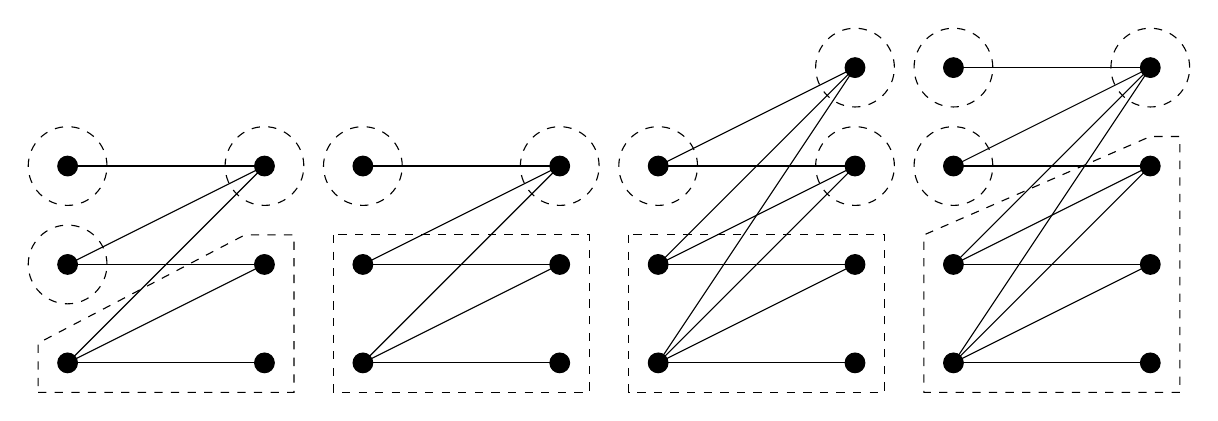
\begin{tikzpicture}
      \tikzstyle{every node}=[font=\fontsize{14.4pt}{18.7pt}\selectfont]
      \draw [ fill={rgb,255:red,0; green,0; blue,0}, fill opacity=1] (7.5,-7) circle (0.125cm);
      \draw [ fill={rgb,255:red,0; green,0; blue,0}, fill opacity=1] (10,-7) circle (0.125cm);
      \draw [ fill={rgb,255:red,0; green,0; blue,0}, fill opacity=1] (10,-8.25) circle (0.125cm);
      \draw [ fill={rgb,255:red,0; green,0; blue,0}, fill opacity=1] (7.5,-5.75) circle (0.125cm);
      \draw [ fill={rgb,255:red,0; green,0; blue,0}, fill opacity=1] (10,-5.75) circle (0.125cm);
      \draw [ fill={rgb,255:red,0; green,0; blue,0}, fill opacity=1] (7.5,-8.25) circle (0.125cm);
      \draw [ fill={rgb,255:red,0; green,0; blue,0}, fill opacity=1] (11.25,-7) circle (0.125cm);
      \draw [ fill={rgb,255:red,0; green,0; blue,0}, fill opacity=1] (13.75,-7) circle (0.125cm);
      \draw [ fill={rgb,255:red,0; green,0; blue,0}, fill opacity=1] (13.75,-8.25) circle (0.125cm);
      \draw [ fill={rgb,255:red,0; green,0; blue,0}, fill opacity=1] (11.25,-5.75) circle (0.125cm);
      \draw [ fill={rgb,255:red,0; green,0; blue,0}, fill opacity=1] (13.75,-5.75) circle (0.125cm);
      \draw [ fill={rgb,255:red,0; green,0; blue,0}, fill opacity=1] (11.25,-8.25) circle (0.125cm);
      \draw [ fill={rgb,255:red,0; green,0; blue,0}, fill opacity=1] (15,-7) circle (0.125cm);
      \draw [ fill={rgb,255:red,0; green,0; blue,0}, fill opacity=1] (17.5,-7) circle (0.125cm);
      \draw [ fill={rgb,255:red,0; green,0; blue,0}, fill opacity=1] (17.5,-8.25) circle (0.125cm);
      \draw [ fill={rgb,255:red,0; green,0; blue,0}, fill opacity=1] (15,-5.75) circle (0.125cm);
      \draw [ fill={rgb,255:red,0; green,0; blue,0}, fill opacity=1] (17.5,-5.75) circle (0.125cm);
      \draw [ fill={rgb,255:red,0; green,0; blue,0}, fill opacity=1] (15,-8.25) circle (0.125cm);
      \draw [ fill={rgb,255:red,0; green,0; blue,0}, fill opacity=1] (18.75,-7) circle (0.125cm);
      \draw [ fill={rgb,255:red,0; green,0; blue,0}, fill opacity=1] (21.25,-7) circle (0.125cm);
      \draw [ fill={rgb,255:red,0; green,0; blue,0}, fill opacity=1] (21.25,-8.25) circle (0.125cm);
      \draw [ fill={rgb,255:red,0; green,0; blue,0}, fill opacity=1] (18.75,-5.75) circle (0.125cm);
      \draw [ fill={rgb,255:red,0; green,0; blue,0}, fill opacity=1] (21.25,-5.75) circle (0.125cm);
      \draw [ fill={rgb,255:red,0; green,0; blue,0}, fill opacity=1] (18.75,-8.25) circle (0.125cm);
      \draw [ fill={rgb,255:red,0; green,0; blue,0}, fill opacity=1] (18.75,-4.5) circle (0.125cm);
      \draw [ fill={rgb,255:red,0; green,0; blue,0}, fill opacity=1] (21.25,-4.5) circle (0.125cm);
      \draw [ fill={rgb,255:red,0; green,0; blue,0}, fill opacity=1] (17.5,-4.5) circle (0.125cm);
      \draw  (7.5,-5.75) -- (10,-5.75);
      \draw  (7.5,-8.25) -- (10,-5.75);
      \draw  (7.5,-8.25) -- (10,-8.25);
      \draw  (10,-7) -- (7.5,-7);
      \draw  (7.5,-7) -- (10,-5.75);
      \draw  (10,-7) -- (7.5,-8.25);
      \draw  (11.25,-5.75) -- (13.75,-5.75);
      \draw  (13.75,-5.75) -- (11.25,-8.25);
      \draw  (11.25,-8.25) -- (13.75,-7);
      \draw  (13.75,-7) -- (11.25,-7);
      \draw  (11.25,-7) -- (13.75,-5.75);
      \draw  (13.75,-8.25) -- (11.25,-8.25);
      \draw  (15,-5.75) -- (17.5,-5.75);
      \draw  (17.5,-7) -- (15,-7);
      \draw  (15,-8.25) -- (17.5,-8.25);
      \draw  (17.5,-4.5) -- (15,-5.75);
      \draw  (17.5,-4.5) -- (15,-7);
      \draw  (17.5,-4.5) -- (15,-8.25);
      \draw  (17.5,-5.75) -- (15,-7);
      \draw  (17.5,-5.75) -- (15,-8.25);
      \draw  (17.5,-7) -- (15,-8.25);
      \draw  (18.75,-4.5) -- (21.25,-4.5);
      \draw  (21.1616,-5.6616) -- (21.1616,-5.6616);
      \draw  (21.25,-5.75) -- (18.625,-5.75);
      \draw  (18.75,-7) -- (21.25,-7);
      \draw  (21.25,-8.25) -- (18.75,-8.25);
      \draw  (18.75,-8.25) -- (21.25,-7);
      \draw  (18.75,-7) -- (21.25,-5.75);
      \draw  (18.75,-5.75) -- (21.25,-4.5);
      \draw  (21.25,-4.5) -- (18.75,-7);
      \draw  (21.25,-5.75) -- (18.75,-8.25);
      \draw  (21.25,-4.5) -- (18.75,-8.25);
      \draw [ dashed] (7.5,-5.75) circle (0.5cm);
      \draw [ dashed] (12,-4.5) circle (0cm);
      \draw [ dashed] (7.5,-5.75) circle (0cm);
      \draw [ dashed] (7.5,-7) circle (0.5cm);
      \draw [ dashed] (10,-5.75) circle (0.5cm);
      \draw [ dashed] (10.875,-6.625) rectangle  (14.125,-8.625);
      \draw [ , dashed] (7.125,-8.625) -- (10.375,-8.625) -- (10.375,-6.625) -- (9.75,-6.625) -- (7.125,-8) -- (7.125,-8.625);
      \draw [ dashed] (11.25,-5.75) circle (0.5cm);
      \draw [ dashed] (13.75,-5.75) circle (0.5cm);
      \draw [ dashed] (17.5,-4.5) circle (0.5cm);
      \draw [ dashed] (17.5,-5.75) circle (0.5cm);
      \draw [ dashed] (15,-5.75) circle (0.5cm);
      \draw [ dashed] (14.625,-6.625) rectangle  (17.875,-8.625);
      \draw [ , dashed] (21.625,-8.625) -- (18.375,-8.625) -- (18.375,-6.625) -- (21.25,-5.375) -- (21.625,-5.375) -- (21.625,-8.625);
      \draw [ dashed] (18.75,-5.75) circle (0.5cm);
      \draw [ dashed] (18.75,-4.5) circle (0.5cm);
      \draw [ dashed] (21.25,-4.5) circle (0.5cm);
    \end{tikzpicture}
  }%
  \caption{The process for building a half-graph}
  \label{fig:half_builder}
\end{figure}